\documentclass{article}
    % General document formatting
    \usepackage[margin=0.7in]{geometry}
    \usepackage[parfill]{parskip}
    \usepackage[T5]{fontenc}
    \usepackage[utf8]{inputenc}
    \usepackage{amsmath}
    \usepackage{tikz}
    \usepackage{fancyhdr}

\pagestyle{fancy}
\fancyhf{}
\rhead{Edgar Jacob Rivera Rios - A01184125}

\begin{document}
a) Show that for any x, $x \in A + B$ iff x is an element of exactly one of A, B
\begin{equation*}
    x \in A + B \implies (x \in A \cap x \notin B) \cup (x \in B \cap x \notin A)
\end{equation*}
\begin{equation*}
    x \in A \cap B \implies x \in A \cap x \in B \implies Not\ in\ A + B
\end{equation*}
b) Draw a Venn diagram for the operation\\
\begin{center}
    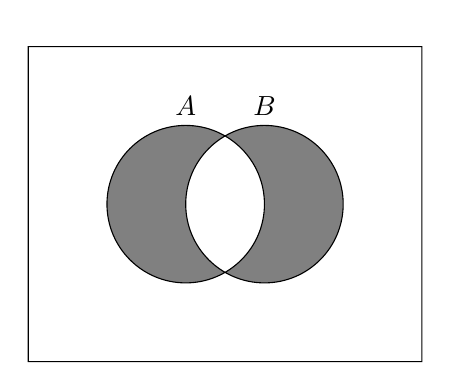
\begin{tikzpicture}[fill=gray]
        % left hand
        \scope
        \clip (-2,-2) rectangle (2,2)
            (1,0) circle (1);
        \fill (0,0) circle (1);
        \endscope
        % right hand
        \scope
        \clip (-2,-2) rectangle (2,2)
            (0,0) circle (1);
        \fill (1,0) circle (1);
        \endscope
        % outline
        \draw (0,0) circle (1) (0,1)  node [text=black,above] {$A$}
            (1,0) circle (1) (1,1)  node [text=black,above] {$B$}
            (-2,-2) rectangle (3,2) node [text=black,above] {};
    \end{tikzpicture}
\end{center}
(c) Show that $A+B \subseteq A \cup B$ \\
\begin{equation*}
    x \in A+B \implies (x \in A \cap x \notin B) \cup (x \in B \cap x \notin A)
\end{equation*}
\begin{equation*}
    x \in A \cup B \implies x \in A \cup x \in B
\end{equation*}
\begin{align*}
    x \in A \cap x \notin B &\implies x \in A\\
                   &\implies x \in A \cup B
\end{align*}
\begin{align*}
    x \in B \cap x \notin A &\implies x \in B\\
                   &\implies x \in A \cup B
\end{align*}
(d) Show that $A+B$ is disjoint from $A \cap B$.\\
\begin{equation*}
    Show\ that\ (A \cap B) \cap (A+B) = \emptyset
\end{equation*}
\begin{equation*}
    x \in A+B \implies (x \in A \cap x \notin B) \cup (x \in B \cap x \notin A)
\end{equation*}
\begin{align*}
    x \in (A \cap B) \cap (A+B) &\implies (x \in A \cap x \in B) \cap ((x \in A \cap x \notin B) \cup (x \in B \cap x \notin A))\\
    &\implies ((x \in A \cap x \notin B) \cap (x \in A \cap x \in B)) \cup ((x \in B \cap x \notin A) \cap (x \in A \cap x \in B))\\
    &\implies (x \in A \cap x \notin B \cap x \in B) \cup (x \in B \cap x \notin A \cap x \in A)\\
    &\implies (x \in A \cap \emptyset) \cup (x in B \cap \emptyset)\\
    &\implies \emptyset \cup \emptyset\\
    &\implies \emptyset
\end{align*}
(e) Show that $A+B = (A \cup B)\setminus(A \cap B)$.\\
\begin{equation*}
    A+B \implies ( A \cap B') \cup (A' \cap B)
\end{equation*}
\begin{align*}
    (A \cup B)\setminus(A \cap B) &\implies ((A \cup B)\setminus A) \cup ((A \cup B)\setminus B)\\
    &\implies (B\setminus A) \cup (A \setminus B)\\
    &\implies (A\cap B') \cup (A' \cap B)
\end{align*}
\begin{equation*}
    A+B = (A \cup B)\setminus(A \cap B)
\end{equation*}
\newpage
(f) For each of the following properties of $\cup$, check out whether or not it also holds for +, giving a proof or a counter example as appropriate: \\
\renewcommand{\labelenumi}{\roman{enumi}}
\begin{enumerate}
    \item commutativity
    \begin{equation*}
        A + B =  B + A
    \end{equation*}
    \begin{equation*}
        x \in A + B \implies (x \in A \cap x \notin B) \cup (x \in B \cap x \notin A)
    \end{equation*}
    \begin{equation*}
        x \in B + A \implies (x \in B \cap x \notin A) \cup (x \in A \cap x \notin B)
    \end{equation*}
    \begin{equation*}
        (x \in A \cap x \notin B) \cup (x \in B \cap x \notin A) = (x \in B \cap x \notin A) \cup (x \in A \cap x \notin B)
    \end{equation*}
    \item associativity
    \begin{equation*}
        (A+B)+C = A+(B+C)
    \end{equation*}
    \begin{align*}
        (A+B)+C &\implies (((A \cap B') \cup (A' \cap B)) \cap C') \cup (((A \cap B') \cup (A' \cap B))' \cap C)\\
        &\implies (((A \cap B') \cup (A' \cap B)) \cap C') \cup (((A \cap B')' \cap (A' \cap B)') \cap C)\\
        &\implies (((A \cap B') \cup (A' \cap B)) \cap C') \cup (((A' \cup B) \cap (A \cup B')) \cap C)\\
        &\implies (A \cap B' \cap C') \cup (A' \cap B \cap C') \cup ((A' \cup B) \cap (A \cup B') \cap C)\\
        &\implies (A \cap B' \cap C') \cup (A' \cap B \cap C') \cup ((A' \cup B) \cap ((A \cap C ) \cup (B' \cap C)))\\
        &\implies (A \cap B' \cap C') \cup (A' \cap B \cap C') \cup (((A' \cup B) \cap (A \cap C )) \cup ((A' \cup B) \cap (B' \cap C)))\\
        &\implies (A \cap B' \cap C') \cup (A' \cap B \cap C') \cup (B \cap A \cap C) \cup (A' \cap B' \cap C)\\
        &\implies (A \cap B' \cap C') \cup (A' \cap B \cap C') \cup (A' \cap B' \cap C) \cup (A \cap B \cap C)
    \end{align*}
    \begin{align*}
        (B+C)+A &\implies (((B \cap C') \cup (B' \cap C)) \cap A') \cup (((B \cap C') \cup (B' \cap C))' \cap A)\\
        &\implies (((B \cap C') \cup (B' \cap C)) \cap A') \cup (((B \cap C')' \cap (B' \cap C)') \cap A)\\
        &\implies (((B \cap C') \cup (B' \cap C)) \cap A') \cup (((B' \cup C) \cap (B \cup C')) \cap A)\\
        &\implies (B \cap C' \cap A') \cup (B' \cap C \cap A') \cup ((B' \cup C) \cap (B \cup C') \cap A)\\
        &\implies (B \cap C' \cap A') \cup (B' \cap C \cap A') \cup ((B' \cup C) \cap ((B \cap A ) \cup (C' \cap A)))\\
        &\implies (B \cap C' \cap A') \cup (B' \cap C \cap A') \cup (((B' \cup C) \cap (B \cap A )) \cup ((B' \cup C) \cap (C' \cap A)))\\
        &\implies (B \cap C' \cap A') \cup (B' \cap C \cap A') \cup (C \cap B \cap A) \cup (B' \cap C' \cap A)\\
        &\implies (B \cap C' \cap A') \cup (B' \cap C \cap A') \cup (B' \cap C' \cap A) \cup (B \cap C \cap A)\\
        &\implies (A \cap B' \cap C') \cup (A' \cap B \cap C') \cup (A' \cap B' \cap C) \cup (A \cap B \cap C)
    \end{align*}
    \begin{align*}
        x \in (A + B) + C &\implies(x \in A \cap x \notin B \cap x \notin C) \cup (x \notin A \cap x \in B \cap x \notin C) \cup\\
        &\qquad\quad(x \notin A \cap x \notin B \cap x \in C) \cup (x \in A \cap x \in B \cap x \in C)
    \end{align*}
    \begin{align*}
        x \in A + (B + C) &\implies (x \in A \cap x \notin B \cap x \notin C) \cup (x \notin A \cap x \in B \cap x \notin C) \cup\\
        &\qquad\quad(x \notin A \cap x \notin B \cap x \in C) \cup (x \in A \cap x \in B \cap x \in C)
    \end{align*}
    \item distribution of $\cap$ over +
    \begin{equation*}
        A \cap (B + C) = (A \cap B) + (A \cap C)
    \end{equation*}
    \begin{align*}
        (A \cap B) + (A \cap C) &\implies ((A \cap B) \cap (A \cap C)') \cup ((A \cap B)' \cap (A \cap C))\\
        &\implies ((A \cap B) \cap (A' \cup C')) \cup ((A' \cup B') \cap (A \cap C))\\
        &\implies ((A \cap B) \cap A') \cup ((A \cap B) \cap C') \cup (A'\cap (A \cap C)) \cup (B' \cap (A \cap C))\\
        &\implies ((\emptyset) \cup ((A \cap B) \cap C') \cup (\emptyset) \cup (B' \cap (A \cap C))\\
        &\implies (A \cap B \cap C') \cup (A \cap B' \cap C)\\
        &\implies A \cap ((B \cap C') \cup (B' \cap C))\\
        &\implies  A \cap (B + C)
    \end{align*}
    \item distribution of + over $\cap$
    \begin{equation*}
        A + (B \cap C) \neq (A + B) \cap (A + C)
    \end{equation*}
    \begin{align*}
        A + (B \cap C) &\implies (A \cap (B \cap C)') \cup (A' \cap (B \cap C))\\
        &\implies (A\cap (B' \cup C')) \cup (A' \cap B \cap C)\\
        &\implies (A\cap B') \cup (A\cap C') \cup (A' \cap B \cap C)
    \end{align*}
    \begin{align*}
        (A + B) \cap (A + C) &\implies ((A \cap B')\cup(A'\cap B)) \cap ((A\cap C')\cup(A'\cap C))\\
        &\implies ((A \cap B')\cup A')\cap ((A \cap B')\cup B) \cap ((A\cap C')\cup A')\cap ((A\cap C')\cup C)\\
        &\implies (A \cup A') \cap (B' \cup A')\cap (A\cup B) \cap (B' \cup B) \cap (A \cup A') \cap (C' \cup A')\cap (A\cup C) \cap (C' \cup C)\\
        &\implies (U) \cap (B' \cup A')\cap (A\cup B) \cap (U) \cap (U) \cap (C' \cup A')\cap (A\cup C) \cap (U)\\
        &\implies (A\cup B) \cap (A\cup C) \cap (B' \cup A') \cap (C' \cup A')\\
        &\implies (A \cup (B \cap C)) \cap (A' \cup (B' \cap C'))\\
    \end{align*}
    \begin{align*}
        x \in A \cap B \cap C' &\implies x \in A+(B \cap C)\\
        &\implies x \notin (A + B) \cap (A + C)
    \end{align*}
\end{enumerate}
(g) Express $-(A+B)$ using union, intersection and complement.\\
\begin{align*}
    -(A+B) &\implies -((A|B) \cup (B|A))\\
           &\implies ((A \cap B') \cup (B \cap A'))'\\
           &\implies (A \cap B')' \cap (B \cap A')'\\
           &\implies (A' \cup B) \cap (B' \cup A)\\
           &\implies ((A' \cup B) \cap B') \cup ((A' \cup B) \cap A)\\
           &\implies (A' \cap B') \cup (B \cap B') \cup (A' \cap A) \cup (B \cap A)\\
           &\implies (A' \cap B') \cup (\emptyset) \cup (\emptyset) \cup (B \cap A)\\
           &\implies (A \cap B) \cup (A' \cap B')\\
\end{align*}
(h) We have seen that each of intersection, union and difference corresponds to a truth-functional logical connective. To what connective mentioned in this lecture does symmetric difference correspond? Draw its truth table.
\begin{table}[h!]
    \label{tab:table1}
    \centering
    \begin{tabular}{c|c|c}
        \textbf{A} & \textbf{B} & \textbf{$A+B$}\\
        \hline
        1 & 1 & 0\\
        \hline
        1 & 0 & 1\\
        \hline
        0 & 1 & 1\\
        \hline
        0 & 0 & 0\\
    \end{tabular}
\end{table}
\end{document}